% -*- mode: fundamental -*-

\documentclass[11pt]{article}

% ================================================================
\usepackage[latin1]{inputenc}
\usepackage[T1]{fontenc}
\usepackage{latexsym}
\usepackage{makeidx}
\usepackage{alltt}
\usepackage{verbatim}
\usepackage{fancyvrb}
% \usepackage{moreverb}
\usepackage{ae}
\usepackage{aecompl}

  \usepackage[pdftex,colorlinks=true,bookmarksopen, pdfstartview=FitH,
              linkcolor=blue, citecolor=blue, urlcolor=blue]{hyperref}
  \pdfcompresslevel=9
  \usepackage[pdftex]{graphicx}

% ================================================================

% HORIZONTAL MARGINS
% Left margin, odd pages: 1.00 inch (0.00 + 1)
\setlength{\oddsidemargin}{0.00in}
% Left margin, even pages: 1.00 inch (0.00 + 1)
\setlength{\evensidemargin}{0.00in}
% Text width 6.5 inch (so other margin is 1.00 inch).
\setlength{\textwidth}{6.5in}
% ----------------
% VERTICAL MARGINS
% Top margin 0.5 inch (-0.5 + 1)
\setlength{\topmargin}{-0.5in}
% Head height 0.25 inch (where page headers go)
\setlength{\headheight}{0.25in}
% Head separation 0.25 inch (between header and top line of text)
\setlength{\headsep}{0.25in}
% Text height 9 inch (so bottom margin 1 in)
\setlength{\textheight}{9in}
% ----------------
% PARAGRAPH INDENTATION
\setlength{\parindent}{0in}
% SPACE BETWEEN PARAGRAPHS
\setlength{\parskip}{\medskipamount}
% ----------------
% STRUTS
% HORIZONTAL STRUT.  One argument (width).
\newcommand{\hstrut}[1]{\hspace*{#1}}
% VERTICAL STRUT. Two arguments (offset from baseline, height).
\newcommand{\vstrut}[2]{\rule[#1]{0in}{#2}}
% ----------------
% HORIZONTAL LINE ACROSS PAGE:
\newcommand{\hdivider}{\noindent\mbox{}\hrulefill\mbox{}} 
% ----------------
% EMPTY BOXES OF VARIOUS WIDTHS, FOR INDENTATION
\newcommand{\hm}{\hspace*{1em}}
\newcommand{\hmm}{\hspace*{2em}}
\newcommand{\hmmm}{\hspace*{3em}}
\newcommand{\hmmmm}{\hspace*{4em}}
% ----------------
% VARIOUS CONVENIENT WIDTHS RELATIVE TO THE TEXT WIDTH, FOR BOXES.
\newlength{\hlessmm}
\setlength{\hlessmm}{\textwidth}
\addtolength{\hlessmm}{-2em}

\newlength{\hlessmmmm}
\setlength{\hlessmmmm}{\textwidth}
\addtolength{\hlessmmmm}{-4em}
% ----------------
% ``TIGHTLIST'' ENVIRONMENT (no para space betwee items, small indent)
\newenvironment{tightlist}%
{\begin{list}{$\bullet$}{%
    \setlength{\topsep}{0in}
    \setlength{\partopsep}{0in}
    \setlength{\itemsep}{0in}
    \setlength{\parsep}{0in}
    \setlength{\leftmargin}{1.5em}
    \setlength{\rightmargin}{0in}
    \setlength{\itemindent}{0in}
}
}%
{\end{list}
}
% ----------------
% ITALICISE WORDS
\newcommand{\ie}{\emph{i.e.,}}
\newcommand{\eg}{\emph{e.g.,}}
\newcommand{\Eg}{\emph{E.g.,}}
\newcommand{\etc}{\emph{etc.}}
\newcommand{\via}{\emph{via}}
\newcommand{\vs}{\emph{vs.}}
% ----------------
% CODE FONT (e.g. {\cf x := 0}).
\newcommand{\cf}{\footnotesize\tt}
% ----------------
% KEYWORDS
\newcommand{\kw}[1]{{\bf #1}}

% ----------------------------------------------------------------
% ----------------------------------------------------------------
% HERE BEGINS THE DOCUMENT

\newcommand{\copyrightnotice}{\copyright 2018-2019 R.S.Nikhil; All Rights Reserved}

% ================================================================

\begin{document}

% ----------------------------------------------------------------

\pagestyle{empty}

\begin{center}

\vspace*{1.5in}

{\LARGE\bf Forvis: A Formal RISC-V ISA Specification}

\vspace{1cm}

{\large\bf A Reading and Extension Guide}

\vspace{2cm}

{\Large \emph{Rishiyur S. Nikhil}} \\

Bluespec, Inc.


\vspace{0.5in}

\copyright{} 2018-2019 R.S.Nikhil

\vspace{1in}

Revision: \today

\vspace{1in}

{\Large\bf *** DRAFT: this document is still being written ***}

\end{center}

% ****************************************************************
% PREFACE AND ACKNOWLEDGEMENTS

\newpage

\pagenumbering{roman}

% ================================================================
% Abbreviations and links

\subsection*{Abbreviations, acronyms and terminology and links}

\begin{tabular}{|l|p{4.5in}|}
\hline
CSR   & Control and Status Register \\
\hline
FPR   & Floating Point Register \\
\hline
GPR   & General Purpose Register \\
\hline
Hart  & Hardware Thread.  Not to be confused with software threads
         such as POSIX threads, ``pthreads'', and processes.
	 A hart has, in hardware, its own PC and fetch unit,
	 and can work concurrently with other harts \\
\hline
ISA   & Instruction Set Architecture \\
\hline
PC    & Program Counter \\
\hline
RVWMO & RISC-V Weak Memory Ordering (default memory model) \\
\hline
RZtso & RISC-V Optional TSO Weak Memory Model \\
\hline
spec  & Specification \\
\hline
Sv32  & Virtual Memory System in RV32 systems \\
\hline
Sv39  & Virtual Memory System in RV64 systems \\
\hline
Sv48  & Optional additional Virtual Memory System in RV64 systems \\
\hline
WMM  & Weak Memory Model \\
\hline
\end{tabular}

\vspace*{1cm}

For more information on terminology and concepts, and information on RISC-V, we recommend these fine books:

\begin{itemize}
\item
``The RISC-V Reader: An Open Architecture Atlas'', by Patterson and Waterman~\cite{Patterson2017b}

\item
``Computer Architecture: A Quantitative Approach'', by Hennessy and Patterson~\cite{Hennessy2017}

\item
``Computer Organization and Design: The Hardware/Software Interface'' (RISC-V Edition) by
     Patterson and Hennessy~\cite{Patterson2017a}
\end{itemize}

and the RISC-V Foundation web site: \verb|https://riscv.org|

% ----------------------------------------------------------------

\subsection*{Thanks ...}

\begin{tightlist}

\item to the original creators of RISC-V for making all this possible in the first place.

\item to Bluespec, Inc. for supporting this work.

\item to the RISC-V Foundation for recognizing the importance of formal
specs and constituting the ISA Formal Specification Technical Group.

\item to the members of the RISC-V Foundation's ISA Formal
Specification Technical Group with whom we have wonderful weekly
discussions on this topic.

\item to reviewers who provided feedback on this document: Greg Sullivan, ...

\end{tightlist}


% ****************************************************************
% TABLE OF CONTENTS

\newpage

\pagestyle{myheadings}

\markboth{CONTENTS}{}

{\small

\tableofcontents

}

\pagenumbering{arabic}

% ****************************************************************

\newpage

\begin{center}

\vspace*{4in}

{\Large\emph{This page is intentionally blank.}}

\vspace*{1.5in}


\includegraphics[width=2in]{Figs/MagrittePipe.jpg}

{\small ``This is not a pipe''. Ren� Magritte, 1929.

{https://en.wikipedia.org/wiki/The\_Treachery\_of\_Images}\footnote{
Image from Wikipedia and used with same ``fair use'' rationale:
 {https://en.wikipedia.org/wiki/File:MagrittePipe.jpg}}}

\end{center}


% ****************************************************************

\newpage

\setcounter{page}{1}
% \renewcommand{\thepage}{\arabic{page}}
\markboth{}{Forvis Reading Guide \copyrightnotice}

% ****************************************************************

\section{Introduction}

\label{sec_intro}

Forvis is a formal specification of the RISC-V Instruction Set
Architecture (ISA), and is written in an ``extremely elementary''
subset of the functional programming language Haskell.  The spec is
located in the \verb|src/| directory of this GitHub repository: \\
\hmm \verb|https://github.com/rsnikhil/Forvis_RISCV-ISA-Spec|

Most of this document is merely a set of ``temporary training wheels''
to help read the spec (Haskell source code files), for those new to
Forvis, Haskell, ISAs, or RISC-V.  For many people (especially those
familiar with Haskell), this document may be unnecessary; just viewing
Fig.~\ref{Fig_Overview} to see how the files are organized may be
enough preparation to jump into the code.  The code has copius
comments and can be read on its own.  In any case, this document is
just an assist---it should only be read side-by-side with the code
opened in your favorite code browser.\footnote{All code fragments in
this document are in fact automatically extracted from the actual spec
code.}

Appendix~\ref{sec_extending_forvis} is a guide for those who would
like to extend Forvis with new ISA features (e.g., an ISA extension
like Vectors, Bit Manipulation, etc.)

Appendix~\ref{sec_accelerators} is a guide for those who are not
extending the RISC-V spec \emph{per se}, but would like to use Forvis
simulation as a driver for a new memory-mapped I/O device or
accelerator.

% ================================================================

\subsection{Code overview}

Fig.~\ref{Fig_Overview} shows an overview of many of the source
files.\footnote{For every Haskell module {\tt Foo} in the figure,
you'll find a file {\tt src/Foo.hs} in the repository.}

\begin{figure}[htbp]
    \centering
    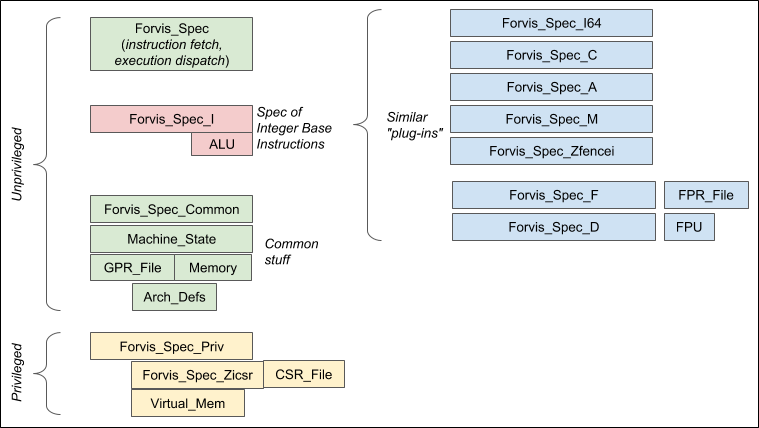
\includegraphics[width=6in]{Figs/Fig_Overview}
    \caption{\label{Fig_Overview}
                    Overview of Forvis files/modules}
\end{figure}

\begin{tightlist}

\item The modules shown in green are common resources used across all instructions.

\item \verb|Forvis_Spec_I|, shown in red, is the base integer
instruction set.  The modules shown in blue are for the other
extensions. All of these files follow exactly the same internal
organization so understanding \verb|Forvis_Spec_I| should help in
understanding them.

\item The modules shown in yellow are the Privileged Architecture.

\end{tightlist}

Please skip to Sec.\ref{sec_common_stuff} to dive into the technical
stuff.  The rest of Sec.~\ref{sec_intro} contains optional detail and
background context.

If you are familiar with Haskell, this code overview may be sufficient
for you to read the code on its own; you may not need the rest of this
document at all.

% ================================================================

\subsection{What is Forvis?}

Forvis cover all these standard RISC-V features and extensions:

\begin{center}
\begin{tabular}{|l|l|}
\hline
RV32I and RV64I  & Base integer instruction sets for RV32 and RV64 \\
\hline
Extension C      & Compressed (16-bit) instructions \\
\hline
Extension A      & Atomic memory operations \\
\hline
Extension M      & Integer multiply and divide instructions \\
\hline
Extension F      & Single-precision Floating Point instructions \\
\hline
Extension D      & Double-precision Floating Point instructions \\
\hline
Extension Zicsr  & CSR (Control and Status Registers) read and write instructions\\
\hline
Extension Zifencei  & FENCE.I instruction \\
\hline
Privileged Architecture  & Machine, Supervisor and User privilege levels \\
                         & Sv32, Sv39 and Sv48 Virtual Memory schemes \\
			 & Exceptions (Traps and Interrupts) \\
\hline
\end{tabular}
\end{center}

The Forvis spec is written in the pure functional programming language
Haskell~\cite{PeytonJones2003} (cf. {\tt haskell.org}) because of its
clean and precise mathematical semantics.

We have deliberately restricted ourselves to an extremely elementary
subset of Haskell so that, along with this reading guide, it is easily
accessible to people who may be totally unfamiliar with Haskell and
who may have no interest in learning Haskell.  Hopefully, familiarity
with types and functions in almost any other programming language
should be adequate background.  In any case, we have also included a
small ``cheat sheet'' in Appendix~\ref{sec_haskell_cheat_sheet} for
the Haskell subset we use.

Using extremely elementary Haskell will also make it easier for authors of
new ISA extensions to extend Forvis to cover their ISA extensions,
even if they are unfamiliar with Haskell.
Appendix~\ref{sec_extending_forvis} provides some guidance on how to
extend Forvis.

Using extremely elementary Haskell will also make it easy to parse and
connect to other tools, such as proof assistants, theorem provers, and
so on.  A parser for Forvis is under development to facilitate this.

% ================================================================

\subsection{Sequential and Concurrent Interpretation as a RISC-V simulator}

\label{sec_sequential_and_concurrent}

Forvis can be directly compiled in Haskell and executed as a RISC-V
simulator where it, in turn, executes RISC-V machine code produced by
hand or by RISC-V assemblers and compilers (the README in the GitHub
repository has directions for how to do this).  This models
{\bf\emph{sequential}}, one-instruction-at-a-time, single-hart
semantics, and is adequate for many (if not most) use-cases.

In contrast, a {\bf\emph{concurrent}} interpretation is required to
model some implementations with advanced micro-architectural features
such as pipelining, separate instruction and data channels to memory,
caches, store buffers, TLBs in MMUs, VLIW and super-scalarity,
out-of-order execution, multi-harts cores and multi-cores.  One may at
first imagine these to be implementation details that would/should be
invisible in an abstract semantics, but in fact their effects are
\emph{deliberately} made visible\footnote{For hardware performance
reasons.} in user programs in certain controlled ways, resulting in
spec features such as ``fence'' instructions and weak memory models.

The Forvis source code, instead of being run through Haskell, can also
be run through an aternative \emph{concurrent} interpreter.  The basic
spec source codes (all the files of form {\tt
Forvis\_Spec\_{\it{}X}.hs}) remain untouched and are used as-is.  What
changes is the infrastructure framework within which that code is
interpreted:
\begin{tightlist}

\item register files change to allow concurrent, out-of-order access;

\item the memory model changes to allow concurrent, out-of-order access;

\item the outer fetch-and-execute loop changes to allow concurrent fetches and executions; etc.

\end{tightlist}

At time of writing, this alternate concurrent interpreter for the same
spec source code is still in development.  It is based on ideas from
``implicit dataflow'' languages and interpretation (cf.  ``Implicit
Parallel Programming in \emph{pH}''\cite{Nikhil2000a}).

% ================================================================

\subsection{Optional background context: Forvis goals}

This is a work-in-progress, one of several similar concurrent efforts
within the ``ISA Formal Specification'' Technical Group constituted by
The RISC-V Foundation ({\tt https://riscv.org}).  The original
English-language specs for RISC-V are:
\begin{itemize}

\item {\it The RISC-V Instruction Set Manual, Volume I: Unprivileged ISA},
    Andrew Waterman and Krste Asanovic,
    Document Version 20181106-Base-Ratification,
    November 6, 2018.~\cite{Waterman2018_user}

\item {\it The RISC-V Instruction Set Manual, Volume II: Privileged
    Architecture}, 
    Andrew Waterman and Krste Asanovic (eds.),
    Document Version 20181203-Base-Ratification,
    December 3, 2018.~\cite{Waterman2018_priv}:

\end{itemize}

Forvis is a formal specification of those specs, i.e., it is written
in a precise, unambiguous language (here, Haskell) without regard to
hardware implementation considerations; clarity and precision are
paramount concerns.  In contrast, specs written a natural language
such as English are often prone to ambiguity, inconsistency and
incompleteness.  Further, a formal spec can be parsed and processed
automatically, connecting to other formal analysis and transformation
tools.  In addition to precision and completeness, Forvis also has
these goals:

\begin{itemize}

\item {\bf Readability:} This spec should be readable by people who
may be completely unfamiliar with Haskell or other formal
specification languages.  Examples of our target audience:

  % ----------------
  \begin{tightlist}
   \item RISC-V Assembly Language programmers as a reference explaining the instructions they use.

   \item Compiler writers targeting RISC-V, as a reference explaining the instructions they generate.

   \item RISC-V CPU hardware designers, as a refernce explaining the instructions interpreted by their designs.

   \item Students studying RISC-V.

   \item Designers of new RISC-V ISA extensions, who may want to
   extend these specs to include their extensions.

   \item Users of formal methods, who wish to prove properties
   (especially correctness) of compilers and hardware designs.

  \end{tightlist}
  % ----------------

\item {\bf Modularity:} RISC-V is one of the most modular ISAs.  It
supports:

  % ----------------
  \begin{tightlist}

   \item A couple of base ISAs: RV32I (32-bit integers) and RV64I
     (64-bit integers) (an RV128I base is under development)

   \item Numerous extensions, such as M (Integer Multiply/Divide), A
    (Atomic Memory Ops), F (single precision floating point), D
    (double precision floating point), C (compressed 16b insructions), E (embedded).

   \item An optional Privilege Architecture, with M (machine) and
    optional S (supervisor) and U (user) privilege levels.

   \item Implementation options, such as whether misaligned memory
   accesses are handled or cause a trap, whether interrupt delegation
   is supported or not, etc.

  \end{tightlist}
  % ----------------

  Implementations can combine these flexibly in a 'mix-and-match'
  manner.  Some of these options can coexist in a single
  implementation, and some may be dynamically switched on and off.
  Forvis tries to capture all these possibilities.

\item {\bf Concurrency and non-determinism:} RISC-V, like most modern
ISAs, has opportunities for concurrency and legal non-determinism.
For example, even in a single hart (hardware thread), it is expected
that most implementations will have pipelined (concurrent) fetch and
execute units, and that the instructions returned by the fetch unit
may be unpredictable after earlier code that writes to instruction
memory, unless mediated by a FENCE.I instruction.  RISC-V has a Weak
Memory Model, so that in a multi-hart system, memory-writes by one
hart may be ``seen'' in a different order by another hart unless
mediated by FENCE and AMO instructions.  In particular, different
implementations, and even different runs of the same program on the
same implementation, may return different results from reading memory
on different runs.

\item {\bf Executabality:} Forvis constitutes an ``operational''
semantics (as opposed to an ``axiomatic'' semantics).  The spec can
actually be executed as a Haskell program, representing a RISC-V
``implementation'', i.e., it can execute RISC-V binaries.  The README
file in the code repository explains how to execute the code.

\end{itemize}

% ****************************************************************

\section{Common Stuff (shared by the various instruction specs)}

\label{sec_common_stuff}

Our tour will go somewhat bottom-up with respect to
Fig.~\ref{Fig_Overview}, first covering some ``common stuff'' used by
all instructions, then the base integer instruction set, then the
top-level instruction fetch and execute semantics.

Reminder: please only read this document side-by-side with the actual code.

% ================================================================

\subsection{File {\tt Arch\_Defs.hs}: basic architectural definitions}

\label{sec_arch_defs}

% ================================================================

\subsubsection{Base ISA type}

The following defines a data type {\tt RV} with two possible values,
{\tt RV32} and {\tt RV64}.  It is analogous to an ``enum'' declaration
in C, defining a family of constants.  The {\tt deriving} clause says
that Haskell can automatically extend the equality operator {\tt ==}
to work on values of type {\tt RV}, and that Haskell can automatically
extend the {\tt show()} function to work on such values, producing
printable Strings {\tt "RV32"} and {\tt "RV64"}, respectively.

\input{Extracted/RV.tex}

% ================================================================

\subsubsection{Key architectural types: instructions and registers}

Througout the spec, we use Haskell's ``unbounded integer'' type
(\verb'Integer') to represent values that are typically represented in
hardware as bit vectors of fixed size.  Unbounded integers are truly
unbounded and have no limit such as the typical 32 bits or 64 bits
found in most programming languages.  Unbounded integers never
overflow. In this spec, we take care of 32-bit and 64-bit overflow
explicitly (inside module \verb|ALU|).

Below, we define Haskell ``type synonyms'' as more readable synonyms
for Haskell's {\tt Integer} type.

\input{Extracted/Instr.tex}

This Haskell function decides whether a particular instruction is a
32-bit instruction or a 16-bit (compressed) instruction, by testing
its two least-significant bits.

\input{Extracted/is_instr_C.tex}

Here, and everywhere in the spec, you can safely ignore the
\verb|INLINE| annotation.  These are ``pragmas`` or ``directives'' to
the Haskell compiler when we compile this spec into a sequential
simulator, and are purely meant to improve the performance (speed) of
the simulator.  In accordance with the their semantic unimportance, we
write these \verb|INLINE| annotations \emph{below} the corresponding
function.

% ================================================================

\subsubsection{Major Opcodes for 32-bit instructions}

The 7 least-significant bits of a 32-bit instruction constitute its
``major opcode''.  This section defines them for the base ``I''
instruction set.

\input{Extracted/Major_Opcodes.tex}

Later in the file, we see major-opcode definitions for the ``A''
(Atomics) extension\footnote{I am grateful to my colleague Joe Stoy
for teaching me the etymology of the word ``atomic''.  It can be read as
``a+tom+ic''.  The ``tom'' (as in ``tomography'') means ``cut'', and
the ``a`` negates it ($\rightarrow$ ``uncuttable'').}, the ``F'' and
``D'' extensions (single-precision and double floating point).

Most instructions also have other fields that further refine the
opcode; we call them ``sub-opcodes''.  These are generally defined in
the separate modules for each extention because they are only used
locally there (for example, in a section labelled ``Sub-opcodes for
'I' instructions'' in file \verb|Forvis_Spec_I.hs|).

However, some sub-opcodes are used in multiple modules and are
therefore defined in this file (\verb|Arch_Defs.hs|).  These include
all the memory-operation sub-opcodes such as \verb|funct3_LB|,
\verb|funct3_SB|, \verb|msbs5_AMO_ADD|, etc., as well as
\verb|funct3_PRIV|.

% ================================================================

\subsubsection{Exception Codes}

We define a type synonym for exception codes, and the values of all
the standard exception codes for traps:

\input{Extracted/exception_codes_B}

and for interrupts:

\input{Extracted/exception_codes_A}

% ================================================================

\subsubsection{Memory responses}

\label{sec_mem_responses}

We define a type {\tt Mem\_Result} for responses from memory.  This
may be {\tt Mem\_Result\_Ok} (successful), in which case it returns a
value (irrelevant for STORE instructions, but relevant for LOAD,
load-reserved, store-conditional, and AMO ops).  Otherwise it is a
{\tt Mem\_Result\_Err}, in which case it returns an exception code
(such as misalignment error, an access error, or a page fault.)

\input{Extracted/Mem_Result}

When returning a result, we construct result-expressions like this:
\begin{tabbing}
\hmmm \= {\tt Mem\_Result\_Ok} \hm \= \emph{value-expression} \\
      \> {\tt Mem\_Result\_Err}    \> \emph{exception-value-expression}
\end{tabbing}

When fielding a result, we deconstruct it using a case-expression like this:
\begin{tabbing}
\hmmm \= {\tt case} mem-result {\tt of} \\
      \> \hm \= {\tt Mem\_Result\_Ok} v \hm {\tt ->} \= \emph{use} v \emph{in an expression} \\
      \>     \> {\tt Mem\_Result\_Err} ec   {\tt ->} \> \emph{use} ec \emph{in an expression}
\end{tabbing}

% ================================================================

\subsection{File {\tt GPR\_File.hs}: General Purpose Registers}

\label{sec_gprs}

This module implements a file of general-purpose registers.  We
represent it using Haskell's \verb|Data_Map.Map| type, which is an
associative map (like a Python ``dictionary'') that associates
register names with values).  This representation choice is purely
internal to this module because we only ever access it via the API
functions in this file, i.e., we treat it like an \emph{abstract data
type}.  Here is the representation and constructor:

\input{Extracted/GPR_File}

The \verb|zip| function constructs a listof intial values, associating
each register address (0..31) with 0 (arbitrarily chosen, since the
spec does not specify the initial value of any register).

This is followed by the API functions \verb|gpr_read| and
\verb|gpr_write|.  The latter always writes 0 into GPR 0, so we can
only ever read 0 from GPR 0.\footnote{In ``{\tt seq~val1~(..)}'' in
the last line of {\tt gpr\_write}, only the part in parentheses is
relevant, doing the actual GPR register file update; the rest is a
wrapper that is merely a Haskell performance optimization for the
simulator, concerned with Haskell's lazy evaluation regime.}

Note: we do not here model accesses to the register file that
concurrent, interleaved, and returning results out of order.  This is
fine for sequential interpretation, but will have to be enriched for
concurrent interpretation.

% ================================================================

\subsection{File {\tt Memory.hs}: Memory}

\label{sec_memory}

This module implements a model of memory.  We represent it using
Haskell's \verb|Data_Map.Map| type, which is an associative map (like
a Python ``dictionary'') that associates addresses with values).  This
representation choice is purely internal to this module; for all other
modules it is an abstract data type accessible only via the API we
export from this module (so we can freely change the internal
representation, in future, if we wish).

Here is the representation and constructor:

\input{Extracted/Memory}

[In anticipation of supporting the 'A' ISA option (atomics), we also
have a field that ``remembers'' the address of the most recent
Load-Reserved instruction, to be matched against the next
Store-Conditional instruction.]

The constructor's argument is a list of (address, byte) pairs, and it
initializes the data map with those contents.  As a practical
simulation-speed consideration, we represent memory in 32-bit words
(even though it is byte-addressable) since most accesses are at 32-bit
or 64-bit granularity (even in RV64, instruction accesses are at
32-bit granularity).

Later in the file we see the API to read memory:

\input{Extracted/mem_read}

and to write memory:

\input{Extracted/mem_write}

In both cases, the first argument is the memory itself, the second
argument (\verb|funct3| is the same 3-bit value in the original LOAD
or STORE instruction indicating the size of the access (byte,
halfword, word or doubleword).  The third argument is the memory
byte-address and the \verb|mem_write| function has a fourth argument
which is the store-value.

The internal details are not too interesting; they're doing some
bit-manipulation to accommodate the fact that our representation is in
4-byte words, and the access size may be for 1, 2, 4 or 8 bytes.

The last fragment of the function checks if the access is aligned:

\input{Extracted/mem_read_aligned}

and returns an exception result if so.  A future version of this spec
will make this a parameter, since an implementation is allowed to
handle misaligned accesses directly (and not return an exception).

Later in the file you will also see the function \verb|mem_amo| that
handles read-modify-write operations in the ``A'' (atomics) extension,
but you can ignore it for now while we focus on the base Integer
instruction set.

Note: we do not model caches, or write-buffers, or any such hardware
implementation artifact here.  This is fine for sequential
interpretation, but will have to be enriched for concurrent
interpretation.

% ================================================================

\subsection{File {\tt Machine\_State.hs}: architectural and machine state}

\label{sec_machine_state}

[Reminder: this is for the simple, sequential,
one-instruction-at-a-time interpreter.  The concurrent interpreter has
a substantially different machine state.]

% ================================================================

\subsubsection{Handling RV32 and RV64 simultaneously}

Although hardware implementations are typically either RV32 systems or
RV64 systems, the spec encompasses implementations that can
simultaneously support both.  For example, machine-privilege code may
run in RV64 mode while supervisor- and user-privilege code may run in
RV32 mode.  There is also a future RV128 being defined.

In Forvis, which covers RV32 and RV64 and their simultaneous use, we
represent everything using unbounded integers (Haskell's
``\verb|Integer|'' type).  The semantics of each instruction are
defined to be governed by the current RV setting which is available in
the architectural state (specifically, MISA.MXL, MSTATUS.SXL,
MSTATUS.UXL, etc.).  RV32 has a smaller integer instruction set than
RV64, and limits calculations on values to 32-bit arithmetic.

% ================================================================

\subsubsection{Machine State}

We define a new type representing a \emph{complete} ``machine state''.
The representation is a record (or struct).

\input{Extracted/Machine_State}

The first few fields represent a RISC-V hart's basic architectural
state: a Program Counter, general purpose registers, floating-point
regsiters, control-and-status Registers, and the current privilege
level at which it is running. This is followed by two fields
representing memory and memory-mapped I/O devices.\footnote{We have
not yet discussed FPRs, CSRs and MMIO, but they can be ignored for now
while we focus on the base Integer instruction set.}

Finally, we have fields that are not semantically relevant, but are
needed or useful in simulation or formal reasoning, gathering
statistics, etc., including a list of legal address ranges (memory
load/store instructions should trap if accessing anything outside this
range).

This record-with-fields representation is a choice purely internal to
this module.  Clients of this module only access it via the
\verb|mstate_|{\it{}function} API that follows.\footnote{Haskell has
export-import mechanisms to enforce this external invisibility of our
representation choice, but we have omitted them here to avoid
clutter.}

The following function is a constructor that returns a new machine state:

\input{Extracted/Machine_State_constructor}

The \verb|misa| argument is passed down to the CSR register file
constructor; it can be ignored for now.  The \verb|addr_byte_list| is
passed down into the memory constructor to intialize memory.

All functions that ``update'' the machine state are written in purely
functional style: the last argument is typically a machine state, and
the final result is the new machine state.  This will be evident in
their type signatures:

\begin{tabbing}\tt
\hmm {\it somefunction} :: {\it ...other arguments...} -> Machine\_State -> Machine\_State
\end{tabbing}

For those unfamiliar with functional programming, it is sometimes
startling to see something as ``large'' as a machine state passed as
an argument and returned as a result, but rest assured this is fine
for our spec; these are just like functions in mathematics.

What follows in the file is a series of API functions to read or
update the machine state, such as the following to access and update
the PC:

\input{Extracted/PC_access}

The \verb|mstate_pc_read| function just applies the \verb|f_pc| field
selector to the machine state to extract that field.  The
\verb|mstate_pc_write| function uses Haskell's ``field update''
notation:

\begin{tabbing}\tt
\hmm \verb|mstate { f_pc = val }|
\end{tabbing}
to construct (and return) a new machine state in which the \verb|f_pc|
field has the new value.

Many of the API functions, such as those to read and write GPRs, FPRs
or CSRs merely invoke the appropriate API of the corresponding
component (GPR file, FPR file or CSR file).

In the API functions for read, write and atomic memory operations,
such as \verb|mstate_mem_read|, we check if the given address is a
supported memory address and return an exception if not.  Otherwise,
we triage the address to determine if it is for actual memory or for a
memory-mapped I/O device, and direct the request to the appropriate
component.

The API functions for FENCE, FENCE.I and SFENCE.VMA are currenty
no-ops in the spec since they only come into play when there is
concurrency involving multiple paths to memory from one or more harts
(hardware threads).  For a sequential one-instruction-at-a-time
interpretation, without multiple paths to memory, with just one hart,
it is fine to treat them as no-ops (more accurately, as the identity
function on the machine state).

The file ends with a number of functions to aid in simulation, to move
console input and output between the machine state and the console, to
``tick'' IO devices (which logically run concurrently with the CPU), etc.

% ================================================================

\subsection{File {\tt Forvis\_Spec\_Common.hs}: Common ``instruction-finishing'' functions}

\label{sec_standard_finish_functions}

Although there are dozens of different instruction opcodes (hundreds,
if we count ISA extensions), there are only five or six ways in which
they all ``finish''-- possibly write a value to a destination
register, possibly increment the PC by 2 or 4, or write a new value
into the PC, possibly increment the MINSTRET (number of instructions
retired) register, and so on.

Another possibility is to trap, which does standard things like
storing a cause in the MCAUSE register, storing the current PC in the
xEPC register, deciding whether the next PC should come from the
MTVEC, STVEC or UTVEC register (taking into account delegation in the
MIDELEG and MEDELEG registers), manipulate the MSTATUS register in a
certain stylized manner (``pushing'' the interrupt-enable and
privilege stacks), and so on.

Rather than replicate these few patterns in each instruction's
semantic function, we collect them in this file in standard functions
and just invoke them from each instruction's semantic function.  For
example, this function captures the common finish of all ALU
instructions, which:

\begin{tightlist}

\item write a result value \verb|rd_val| to the GPR \verb|rd|;

\item increment the PC by 4 or 2, depending on boolean \verb|is_C|,
which indicates whether the current instruction is a regular 32-bit
instruction or a 16-bit C (compressed) instruction;

\item and increment the MINSTRET (instructions retired) counter.

\end{tightlist}

\input{Extracted/finish_rd_and_pc_incr}

% ****************************************************************

\section{File {\tt Forvis\_Spec\_I}: Base Integer Instruction Specs}

\label{sec_ISA_spec_I}

We are now ready to look at this module which covers the whole RV32
Integer instruction set.  The organization of the code in this module
is also followed in the modules for other extensions (I64, C, A, M,
Zifencei, F, D, Priv, Zicsr):

\begin{itemize}

\item Declaration of a type \verb|Instr_I|, a data structure
representing all the instructions in this group, along with each one's
logical fields.  This is a Haskell ``algebraic data type''.  These are
like ``abstract syntax trees'' for instructions in this group.

\item Definitions of sub-opcodes for instructions in group I.  These
are values of fields in a 32-bit instruction that collectively refine
it to a more specific instruction opcode.

\item A decode function \verb|decode_I| of type: \\
\hmm \verb|decode_I :: RV -> Instr_32b -> Maybe Instr_I| \\
that takes a a 32-bit instruction and returns a result that is either:
  \begin{tightlist}

    \item \verb|Nothing|: this is not an instruction in this group,

    \item or \verb|Just adt|: this is an instruction in this group,
    and \verb|adt| is a value of the algebraic data type
    \verb|Instr_I|, i.e., the logical view of the instruction.

  \end{tightlist}
  The \verb|RV| argument is because these functions serve for both the
  RV32 and RV64 base integer instructions, but some instructions are
  only valid in RV64.

\item An execution-dispatch function \verb|exec_instr_I| that
dispatches each kind of instruction in the group to a specific
execution function for that particular kind of instruction.

\item A series of functions \verb|exec_LUI|, \verb|exec_AUIPC|,
\verb|exec_JAL|, ..., one per opcode, describing the semantics of that
particular kind of instruction.

\end{itemize}

% ================================================================

\subsection{Algebraic Data Type for I instructions}

The file begins with a Haskell data type declaration for the type
\verb|Instr_I|:

\input{Extracted/Instr_I}

This should be read as follows: ``A value of type \verb|Instr_I| is
\begin{tightlist}

\item \emph{either} a \verb|LUI| instruction, in which case it has two
fields of type \verb|GPR_Addr| and
\verb|InstrField| (the destination register rd and a 20-bit immediate value),

\item \emph{or} a \verb|AUIPC| instruction, in which case it has two
fields of type \verb|GPR_Addr| and \verb|InstrField| (the destination
register rd and a 20-bit immediate value),

\item \emph{or} a \verb|JAL| instruction, in which case it has two
fields of type \verb|GPR_Addr| and \verb|InstrField| (the destination
register rd and a 21-bit immediate value),

\item \emph{or} a \verb|JALR| instruction, in which case it has three
fields of type \verb|GPR_Addr|, \verb|GPR_Addr| and \verb|InstrField|
(the destination register rd, the source register rs1, and a 12-bit
immediate value),

\item ... and so on.''

\end{tightlist}

Note, the width information (20-bit, 21-bit, 12-bit) is just a comment
and is not enforced by type-checking.

% ----------------

\subsection{Sub-opcodes for I instructions}

The next section defines values of other fields in a 32-bit
instruction that further refine the group opcode into a specific
opcode:

\input{Extracted/sub_opcodes_I}

These are values in the 3-bit field in bits [14:12] of a 32-bit instruction.

% ----------------

\subsection{Decoder for I instructions}

The next section defines the function \verb|decode_I| whose arguments
are {\tt rv} (because some I instructions are only valid in RV64 and
not in RV32) and a 32-bit instruction.  The result is of type
\verb|Maybe Instr_I|, i.e., it is:

\begin{tightlist}

 \item \emph{either} \verb|Nothing|: this is not an I instruction,

 \item \emph{or} \verb|Just instr_I|: this is an I instruction, and
 the field \verb|instr_I| is value of type \verb|Instr_I|, the logical
 view of the instruction.

\end{tightlist}

\input{Extracted/decode_I_A}

The first few lines of the function use \verb|bitSlice| to extract
bit-fields of the instruction.  This is a help-function defined in
\verb|Bit_Utils.hs|, and {\tt bitSlice~x~$j$~$k$} is equivalent to the
Verilog/SystemVerilog bit-selection {\tt x[$j$,$k$]}.  Note that some
field-extractions can involve more complex bit-shuffling, such as:

\input{Extracted/decode_I_B}

The decode function essentially abtracts away lower-level details of
how fields are laid out in 32-bit parcels and returns a higher-level,
more abstract view of type \verb|Instr_I|.

The decode function finally defines the result \verb|m_instr_I| (of type
\verb|Maybe Instr_I|) by dispatching on a series of conditions, each
checking for a particular opcode:

\input{Extracted/decode_I_C}

If none of the conditions match, it returns \verb|Nothing|


% ----------------

\subsection{The type of each I-instruction semantic function}

The functions describing the semantics of each I instruction (to
follow, shortly) all have the same type.  In such a situation, it's
good to give a name to this type (using a type-synonym):

\input{Extracted/Spec_Instr_I}

The first argument is a boolean (we'll consistently use the variable
\verb|is_C| for this) indicating whether the current instruction is a
regular 32-bit instruction or a 16-bit (C, compressed) instruction.
In RISC-V, each 16-bit instruction is defined as a ``short form'' for
a specific corresponding 32-bit instruction.  Thus, we define the
semantics in one function, but use the parameter \verb|is_C| to
remember whether we're doing this for a 32-bit or for a 16-bit
instruction.  For almost all instructions, we either update the PC
with the address of the next instruction, or we remember address of
the next instruction (e.g., in JAL and JALR). This
next-instruction-address may be the current PC +2 or +4, depending on
\verb|is_C|.

The second argument is the instruction in its decoded form; the third
argument is the machine state, and the final outcome after executing
the instruction is the new machine state.

% ----------------

\subsection{Dispatcher for I instructions}

The next function is simply a dispatcher that takes an \verb|Instr_I|
value and, based on the kind of I instruction it is, dispatches to a
specific execution function for that kind of of instruction.

\input{Extracted/exec_instr_I}

It uses the Haskell pattern-matching \verb|case| statement to
determine which kind of instruction it is, and invokes the appropriate
function.  Note, it has no check for illegal instructions; the fact
that the argument is of type \verb|Instr_I| guarantees that it can
only be a valid I instruction.

% ----------------

\subsection{Semantics of each I instruction}

This is the meat of instruction semantics: what exactly does each kind
of instruction do?  There is one \verb|exec_|\emph{FOO} function for
each opcode \emph{FOO}.  We examine excerpts of a few of them.  The
first I instruction, LUI, is very simple:

\input{Extracted/exec_LUI}

The second argument is the pattern \verb|(LUI rd imm20)| that is
matched against the instruction, and gives us bindings for the
\verb|rd| and \verb|imm20| fields as a result.  There is no chance
that this pattern fails, since this function is only called by the
dispatcher \verb|exec_instr_I| (above) when it is this kind of
instruction.

It uses the 20-bit immedate to calculate a value \verb|rd_val| to save
in the destination register \verb|rd|, and calls the standard
``finish'' function described in
Sec.~\ref{sec_standard_finish_functions} to write the destination
register and increment the PC, and returns the final machine state.


The \verb|JALR| instruction does a bit more:

\input{Extracted/exec_JALR}

We calculate the saved ``return-address'' (\verb|rd_val| is calculated
as PC+2 or PC+4 depending on \verb|is_C|).  The jump-target PC is
initially calculated by adding the offset to the \verb|rs1_val|.
Then, per the spec, we clear its bit [0] to 0.  Then we check if is is
properly aligned. If MISA.C is active, then it cannot be misaligned
since we just cleared the least-significant bit.  If MISA.C is not
active, then it is aligned only if bits [1:0] are 0.

Finally, if the target is properly aligned, we finish normally
(updating rd and incrementing PC), otherwise we finish by trapping
with exception code \verb|exc_code_instr_addr_misaligned|, and storing
\verb|new_pc'| in the TVAL CSR.

The functions for memory load instructions \verb|exec_LB|,
\verb|exec_LH|, \verb|exec_LW|, \verb|exec_LD| all funnel back through
a common \verb|exec_LOAD| help-function.  Let's focus on this excerpt:

\input{Extracted/exec_LOAD}

It invokes \verb|mstate_vm_read|, which is in file
\verb|Virtual_Mem.hs| (see Sec.~\ref{sec_vm}), which does all memory
reads.  By examining \verb|mstate|, that function can decide whether
the address is a virtual or physical address, and do the translation
if needed.  During translation or subsequent memory access, it may
encounter a fault.  The final result is of type \verb|Mem_Result|
(described in Sec.~\ref{sec_mem_responses}), indicating that it's ok
(and contains the appropriate payload), or an error (and contains the
appropriate exception code).  In the case of an access fault, the
\verb|is_instr| boolean allows the memory system to determine if it
should return an instruction fetch access fault or a load access
fault.

Moving further down the file, the ADD instruction is handled by the
following function:

\input{Extracted/exec_ADD_1}

This just invokes the function \verb|exec_OP| which is used by all the
\verb|opcode_OP| functions.  To this common function, we pass the
function \verb|alu_add| (defined in file \verb|ALU.hs|) to indicate
the specific function to be performed on the operands.

The \verb|exec_OP| function is simple.  We read the Rs1 and Rs2
registers, perform the specified \verb|alu_op|, and finish by updating
the destination register \verb|rd| and incrementing the PC.

\input{Extracted/exec_OP}

Near the end of the file we have the semantics of ECALL:

\input{Extracted/exec_ECALL}

It decides the exception code depending on the current privilege
level, and then finishes with a trap, supplying that exception code,
and 0 for the ``trap value'' (that goes into the xTVAL register).

% ================================================================

\subsection{File {\tt ALU.hs}: A pure integer ALU}

The module \verb|ALU| represents the ``pure integer ALU'', i.e., pure
functions of one or two inputs representing the various integer
arithmetic, logic and comparison operations of interest.  Most of the
functions are quite straightforward, invoking Haskell primitives to
perform the actual operations.

All considerations of whether we are dealing with 32-bit or 64-bit
input and output values, whether they are to be interpreted as signed
or unsigned values, etc., are confined to this module.  Outside this
module, all values are ``stored'' as Haskell's \verb|Integer| data
type.

% ****************************************************************

\section{File {\tt Forvis\_Spec\_Instr\_Fetch.hs}: Instruction Fetch}

\label{sec_instr_fetch}

An instruction fetch can have three possible outcomes, which are
expressed in this data type:

\input{Extracted/Fetch_Result}

The instruction fetch function takes a machine state and returns a
2-tuple: a \verb|Fetch_Result| and a new machine state:

\input{Extracted/instr_fetch}

Note, while we may think of an instruction fetch as a pure ``read'',
we return a potentially changed machine state because even a read can
have side effects.\footnote{For example, a virtual memory access can
change an 'Accessed' bit in a page table entry; a read may be from an
I/O device where reads can have side-effects; if we model caches for
concurrent interpretation, cache state can change; if we model
performance counters, those could change.}

Instruction fetch must be done carefully, avoiding spurious
exceptions.  Consider this scenario: the PC is pointing at the last
two bytes of a virtual memory page.  We do not know whether those two
bytes contain (i) a C instruction, or (ii) the first two bytes of a
normal 32-bit instruction, with PC+2 pointing at its remaining two
bytes.  In case (i), control flow (branches, traps) may never take us
to PC+2, and so we should not unnecessarily read the two bytes there,
in case that read results in a virtual memory exception, being on the
next page.  Thus, we should fetch the latter two bytes \emph{only if
necessary}.

The code for the \verb|instr_fetch| function is structured to handle
this.  It first checks the 'C' flag in CSR MISA to see if compressed
instructions are supported.  If not, it reads a 4-byte (32-bit)
instruction from memory, which may of course return either an
exception or a 32-bit instruction:

\input{Extracted/instr_fetch_1}

If 'C' is supported, it first reads 2 bytes from memory and, if that
is not an exception, checks if it encodes a 'C' instruction:

\input{Extracted/instr_fetch_2}

If it is not a C instruction, then it is the first 2 bytes of a 32-bit
instruction; it reads 2 more bytes from memory and returns it as a
full 32-bit instruction.

% ****************************************************************

\section{File {\tt Forvis\_Spec\_Execute.hs}: Top-level execute function}

\label{sec_execute}

The function \verb|exec_instr_32b| executes exactly one instruction.
It takes an instruction and machine state and returns the updated
machine state resulting from executing that instruction (the second
component of the output 2-tuple, a \verb|String|, is just for printing
out instruction traces during simulation, and has no semantic
significance).  It first calls \verb|decode_I| (and similar decode
functions for other ISA extensions) to decide whether it is an I
instruction and, if so, obtains the abstract version of the
instruction (of type \verb|Instr_I|).

\input{Extracted/exec_instr_32b}

The long list of nested \verb|case| expressions that follow simply
dispatch to the appropriate execution function; for example if it is
an \verb|Instr_I|, it invokes \verb|exec_instr_I|, and so on.

\input{Extracted/exec_instr_32b_3}

At the end of the list of case expressions, i.e., if none of the
decoders identified the instruction, it raises an illegal instruction
exception:

\input{Extracted/exec_instr_32b_5}

The rest of the file is straightforward: the function
\verb|exec_instr_16b| is just like \verb|exec_instr_32b| which we just
examined, except for 16-bit C (compressed) instructions.

% ****************************************************************

\section{Privileged Architecture}

% ================================================================

\subsection{{\tt Arch\_Defs.hs}: Privilege levels}

The privileged architecture instroduces three privilege
levels: Machine, Supervisor and User:

\input{Extracted/Priv_Level}

% ================================================================

\subsection{{\tt Forvis\_Spec\_Priv.hs}: Privileged architecture instructions}

This file follows the standard file organization for each extension/feature:

\begin{tightlist}

\item An algebraic data type \verb|Instr_Priv| for the abstract,
decoded view of privileged architecture instructions;

\item Definitions of sub-opcodes for privileged architecture
instructions, followed by a decode function \verb|decode_Priv|

\item An execution-dispatch function \verb|exec_instr_Priv| from
decoded instructions to individual semantic functions;

\item and, finally, a series of individual semantic functions
\verb|exec_xRET| (for MRET/SRET/ URET), \verb|exec_WFI| and
\verb|exec_SFENCE_VMA|.

\end{tightlist}

% ================================================================

\subsection{File {\tt Forvis\_Spec\_Zicsr.hs}: CSR-GPR atomic swap instructions}

This is the spec for CSR read and write instructions CSRRW, CSRRWI,
CSRRS, CSRRSI, CSRRC, and CSRRCI.  These are technically not part of
the privileged architecture but form their own ``Zicsr'' extension,
but we place this section here here because they are most heavily used
in privileged code.

These instructions atomically read a CSR and place the result in a GPR
while taking another GPR value (or an immediate value) and using it to
write a new value into a CSR.

% ================================================================

\subsection{File {\tt CSR\_File.hs}: Control and Status Registers}

\label{sec_csrs}

Privileged architecture instructions interact heavily with the CSR
register file.  Like the GPR regsiter file, this module's private
representation choice is to use Haskell's \verb|Data.Map|.

The four most-significant bits of a CSR address encode
permissions--whether or not a CSR can be read/written at a particular
privilege level.  The \verb|csr_permission| function computes this
permission, returning None, RO (read-only) or RW (read and write),
which constitute the \verb|CSR_Permission| data type.

The API functions \verb|csr_read| and \verb|csr_write| functions are
the general-purpose access functions for CSRs.  These functions do not
check access permissions; they are only invoked after permissions have
been checked.  Mostly they just access the \verb|Data.Map|, but
several CSR addresses are merely restricted ``views'' of other CSRs,
so these are treated specially before the general lookup/update.

For example,
\begin{tightlist}
\item
\verb|USTATUS| and \verb|SSTATUS| are restricted views of \verb|MSTATUS|

\item
\verb|UIE| and \verb|SIE| are restricted views of \verb|MIE|

\item
\verb|UIP| and \verb|SIP| are restricted views of \verb|MIP|

\item
\verb|FRM| and \verb|FFLAGS| are restricted views of \verb|FCSR|
\end{tightlist}

The file continues with with definitions of CSR addresses and their
reset values, organized into User, Supervisor and Machine privilege
groups.  After these general-purpose definitions, the file continues
with more detailed support for key specific CSRs.

% ================================================================

\subsubsection{The MISA CSR}

A key CSR is MISA (``Machine ISA Register'').  The 2 most-significant
bits are called \verb|MXL| and it encodes the current ``native'' width
of the ISA (width of PC and GPRs), which can be 32, 64 or 128 bits.

\input{Extracted/MISA_fields_A}

The lower 26 bits are named by letters of the alphabet, A-Z, with bit
0 being A and Bit 25 begin Z.  The function \verb|misa_flag|, when
given the value in the MISA register and a letter of the alphabet
(uppercase or lowercase), returns a boolean indicating whether the
corresponding bit is set or not.

\input{Extracted/MISA_fields_B}

This is followed by symbolic-name definitions for the integer bit
positions of the 26 alphabets and the MXL field.

\input{Extracted/MISA_fields_C}

% ================================================================

\subsubsection{The MSTATUS, SSTATUS and USTATUS CSRs}

Another key CSR is MSTATUS (``Machine Mode Status'').  The code for
this section begins with definitions for the integer bit positions of
its fields.  Not all fields are used, and more restricted views of
this CSR are known as SSTATUS (Supervisor Mode Status) and USTATUS
(User Mode Status).  Some ``mask'' definitions encode these views.

This is followed by two help-functions that are used in defining the
semantics of exceptions (interrupts and traps) and
returns-from-exceptions.  The least-significant 8 fields of MSTATUS
represent a shallow ``stack'' of interrupt-enable and privilege
bits. On an exception, we push new values on to this stack, and when
we return-from-exception we pop the stack. The function
\verb|mstatus_stack_fields| extracts the stack, returning the fields
as an 8-tuple: \verb|(mpp,spp,mpie,spie,upie,mie,sie,uie)|.  The
inverse function, \verb|mstatus_upd_stack_fields| takes an MSTATUS
value and an 8-tuple of new stack values, and returns a new MSTATUS
with the stack updated.

The functions \verb|mstatus_stack_fields| and
\verb|mstatus_upd_stack_fields| encapsulate reading and writing the
``stack'' in the MSTATUS register containing the ``previous
privilege'', ``previous interrupt enable'' and ``interrupt enable''
fields.  This stack is pushed on traps/interrupts, and popped on
URET/SRET/MRET instructions.

% ================================================================

\subsubsection{Miscellaneous CSR definitions}

The next several sections have definitions for:

\begin{itemize}

\item The MTVEC, STVEC and UTVEC CSRs: functions to extract the
``mode'' and ``base'' fields of the MTVEC (Machine-level trap vector)
CSR.  The same functions can also be applied to the STVEC and UTVEC
for the Supervisor-level and User-level versions.

\item The MIP, SIP and UIP CSRs: symbolic names for bit positions in
the MIP (Machine-level interrupt pending) CSR.  It also defines masks
for SIP and UIP which are restricted views of the same register at
Supervisor and User privilege levels, respectively.

\item The MCAUSE ``Exception Cause'' CSR: definition of the bit
position that distinguishes interrupts from synchronous traps, for
RV32 and RV64 modes, and a predicate to decide whether an exception
code is for an interrupt of synchronous trap.

\item The FCSR ``floating point status'' CSR: definitions for bit
positions in this CSR.

\end{itemize}


% ================================================================

\subsubsection{Interrupt-pending test and WFI-resumption test}

\label{csr_interrupt_pending}

The function \verb|csr_interrupt_pending| determines if the CSR state
allows taking an interrupt at the current privilege (specifically,
CSRs MISA, MSTATUS, MIP, MIE, MIDELEG, and SIDELEG).

It takes into account the current privilege, whether an interrupt is
pending in the CSR MIP, whether interrupts are delegated to a lower
privilege level (in CSRs MIDELEG and SIDELEG), and whether interrupts
are enabled at the appropriate level (in CSRs MSTATUS/ SSTATUS/
USTATUS and MIE/ SIE/ UIE).  If an interrupt cannot be taken, it
returns \verb|Nothing|; otherwise it returns \verb|Just|~\emph{ec},
where \emph{ec} is the exception code describing the kind of
interrupt.

The function \verb|csr_wfi_resume| returns a boolean indicating
whether the hart is allowed to resume execution if it is currently
waiting at a WFI (Wait For Interrupt) instruction.  The resumption
condition is weaker than the condition used by the previous function
that decides whether we can actually take an interrupt, because it
does not take into account current privilege, delegation, global
(MSTATUS) interrupt-enable fields, and so on.  WFI instructions are
typically used inside a loop where, if the interrupt is not actually
taken, we just come back to wait again at the WFI.

% ================================================================

\subsection{File {\tt Virtual\_Mem.hs}: Virtual Memory}

\label{sec_vm}

This module contains essentially all the code to support virtual
memory, covering the Sv32, Sv39 and Sv48 virtual memory schemes.

Memory access begins in the semantic functions for various memory
access instructions:

\begin{tightlist}

\item \verb|exec_LOAD| and \verb|exec_STORE| in module \verb|Forvis_Spec_I|;

\item \verb|exec_AMO| in module \verb|Forvis_Spec_A|;

\item \verb|exec_FLW| and \verb|exec_FSW| in module \verb|Forvis_Spec_F|;

\item and \verb|exec_FLD| and \verb|exec_FSD| in module \verb|Forvis_Spec_D|.

\item (Compressed memory access instructions, in module
\verb|Forvis_Spec_C| expand to one of the above).

\end{tightlist}

These functions call \verb|mstate_vm_read|, \verb|mstate_vm_write| and
\verb|mstate_vm_amo| in the current file, \verb|Virtual_Mem.hs|.  Each
of these functions first calls \verb|fn_vm_is_active| to check whether
or not we are currently running in a mode that requires
virtual-to-physical translation.  A subtlety is that the current
effective privilege may be modified by the MSTATUS.MPRV and
MSTATUS.MPP bits.

If virtual memory is active, \verb|mstate_vm_read|,
\verb|mstate_vm_write| and \verb|mstate_vm_amo| then call
\verb|vm_translate| which is described later in the file, to translate
the virtual address, returning either a successful translation into a
physical address or an exception (such as a page fault or access
fault).  Note, translation returns an updated memory state because it
may modify the ``access'' and ``dirty'' bits in a page table entry.
Translation is done with a ``page table walk'', which is specified in
the following function:

\input{Extracted/vm_ptw}

This is a recursive function that descends the hierarchy of the page
table, taking into account that any level can point at a leaf page
(page, megapage, gigapage or terapage), and taking into account the
protection bits in Page Table Entries (PTEs).

Hardware implementations typically implement a TLB (Translation
Look-aside Buffer) to cache page-table entries for faster future
access, avoiding repeated page table walks.  However, that is
primarily a performance optimization, and for simplicity we ignore it
here in the semantics and perform the full page-table walk on each
memory access.\footnote{In the concurrent interpretation, cacheing of
PTEs in TLBs must be modeled because it does become observable and
interacts with the SFENCE.VMA instruction.}

The rest of the file contains various help-functions for \verb|vm_translate|.

% ****************************************************************

\section{File {\tt Forvis\_Spec\_Interrupts.hs}: Interrupts}

\label{sec_interrupts}

This module contains two functions related to interrupts.  The
\verb|take_interrupt_if_any| function can be applied between the
execution of any two instructions:

\input{Extracted/take_interrupt}

It first uses the function \verb|csr_interrupt_pending| (described in
Sec.~\ref{csr_interrupt_pending}) to determine if the current machine
state allows taking an interrupt and, if so, which kind of interrupt.

If so, \verb|take_interrupt_if_any| actually ``takes the interrupt'',
i.e., it applies \verb|mstate_upd_on_trap| to update the PC so that
the next instruction fetched will be from the interrupt handler, with
CSRs holding appropriate values for the handler.

If no interrupt can be taken now, it returns \verb|Nothing| and an
unchanged machine state.  The second function in the file is:

\input{Extracted/wfi_resume}

which merely calls \verb|csr_wfi_resume| (also described in
Sec.~\ref{csr_interrupt_pending}) to check if the CPU can resume from
a WFI (Wait For Interrupt) state.  Note, WFI does not actuall take an
interrupt (hence this function does not return any updated machine
state), it merely resumes at the next instruction, which may take the
interrupt (using \verb|mstate_take_interrupt_if_any|).

% ****************************************************************

\section{Sequential (one-instruction-at-a-time)  interpretation}

In Sec.~\ref{sec_sequential_and_concurrent} we discussed how the same
spec code can be \emph{interpreted} in two different ways, sequential
or concurrent.  The file \verb|Run_Program_Sequential.hs| contains the
sequential interpreter, including various hooks to help in simulation
(such as printing out instruction traces).  The main function is this:

\input{Extracted/run_loop}

The \verb|maxinstrs| argument is a simulation aid to limit the number
of instructions executed (stopping runaway simulations).  The
\verb|m_tohost_addr| argument is another simulation aid; it stops
simulation if the CPU writes to a particular location called
\verb|m_tohost_addr|; this facility is used in certain test programs.
The \verb|mstate| argument is the initial machine, when this function
is first called, from the function \verb|run_program_from_files| in
\verb|Main_Run_Program.hs|.

The result returned by \verb|run_loop| is of type
\verb|(Int,Machine_State|).  The first component is a value written
into the \verb|to_host| location if that facility is used to signal
termination, otherwise it is 0.  The second component is the final
machine state.

If we removed the simulation aids, the type of \verb|run_loop| would
be: \\
\hmmm {\tt Machine\_State -> IO Machine\_State} \\
i.e., it simply transforms the machine state by repeatedly executing
instructions.\footnote{ The {\tt IO} type constructor is the Haskell
mechanism by which we can do IO within this loop, such as printing
instruction traces, and reading and writing the console terminal.}
\verb|run_loop| is literally a loop.  The last line of the function:

\input{Extracted/run_loop_1}

shows a tail-recursive call to itself; this is how loops are expressed in Haskell.

The body of \verb|run_loop| does the following (if you scan through
the body ignoring the clutter of simulation aids like printing debug
messages, detecting termination and self-loops, etc.):

\begin{tightlist}

\item it calls \verb|mstate_io_tick| to ``advance'' the conceptually
concurrent processes in I/O devices,

\item it moves console terminal input from the console into the UART
      buffer,

\item it calls the \verb|fetch_and_execute| (later in this file) to
      fetch and execute one instruction,

\item it moves console terminal output from the UART buffer to the
      console,

\item and loops.

\end{tightlist}


% ****************************************************************

\section{Brief Description of Other Spec Source Files}

The list below is in alphabetic order.

% ----------------

\subsection{\tt Bit\_Utils.hs}

This contains utilities for bit manipulation, including bit-field
extraction and concatenation, sign- and zero-extension, truncation,
conversion, etc. that are relevant for these semantics.

% ----------------

\subsection{\tt Forvis\_Spec\_A.hs}

Spec for the ``A'' ISA extension for Atomic memory
operations (Load Reserved, Store Conditional, Atomic swap, add,
and/or/xor, min/max).

% ----------------

\subsection{\tt Forvis\_Spec\_C.hs}

Spec for the ``C'' ISA extension for compressed (16-bit) instructions.

% ----------------

\subsection{\tt Forvis\_Spec\_D.hs}

Spec for the ``D'' ISA extension for double-precision floating point operations.

% ----------------

\subsection{\tt Forvis\_Spec\_F.hs}

Spec for the ``F'' ISA extension for single-precision floating point oeprations.

% ----------------

\subsection{\tt Forvis\_Spec\_I64.hs}

The RV64 base Integer instruction set.

% ----------------

\subsection{\tt Forvis\_Spec\_M.hs}

Spec for the ``M'' extension for integer multiply/divide operations.

% ----------------

\subsection{\tt Forvis\_Spec\_Zifencei.hs}

Spec for the ``Zifencei'' extension for the FENCE.I instruction.

% ----------------

\subsection{\tt FPR\_File.hs}

The floating point register file used by the ``F'' and ``D'' extensions.

% ----------------

\subsection{\tt FPU.hs}

 the floating-point analog of the integer \verb|ALU|
module, representing a ``pure floating point ALU'', encapsulating all
floating-point arithmetic, logic, comparision and conversion
operations. All considerations of single-precision
vs. double-precision, conversions between these and integers etc., are
confined to this module.

% ----------------

\subsection{\tt Mem\_Ops.hs} defines instruction field values that specify the
type and size of memory operations.  These are duplicates of defs in
\verb|Forvis_Spec.hs| where they are in the specs of LOAD, STORE and
AMO instructions.  They are repeated here because this information is
also needed in \verb|Memory.hs|, \verb|MMIO.hs| and other places.

% ****************************************************************

\section{Brief Description of Other Non-Spec Source Files}

These files are not part of the spec \emph{per se}.  They They
represent additional infrastructure to attach the spec (which just
represents a CPU) with a minimal but complete ``system''.
Collectively, they can be compiled and linked as a Haskell executable
that is a RISC-V simulator, for the \emph{sequential} interpretation.
System elements include a boot ROM, a memory, a memory-mapped timer
(MTIME, MTIMECMP), a memory-mapped place to request software
interrupts (MSIP), a serial communication device for the console
(UART), etc.  These are sometimes collectively referred to as a
``platform''.

The list below is in alphabetic order.

% ----------------

\subsection{\tt Address\_Map.hs}

specifies the range of addresses for supported main memory, boot ROM
memory, memory-mapped I/O, and specific memory-mapped addresses for
MTIME. MTIMECMP, MSIP, the UART (serial console communications
device), etc.

% ----------------

\subsection{\tt Elf.hs}

This contains functions for reading ELF files representing RISC-V
executable programs.  Assemblers, compilers and linkers (such as gcc
and llvm) produce ELF files as their output (see also
\verb|Read_Mem_Hex.hs| below).

% ----------------

\subsection{\tt Main.hs}

This is the ``main'' program compiled by the Haskell compiler.  It
contains several alternative use-cases, one of which is statically
chosen by editing this file and ensuring that we comment-out all but
one alternative.

\begin{tightlist}

\item \verb|Main_RunProgram.hs|: a free-running RISC-V simulator.
Reads RISC-V binaries (ELF or Mem Hex), initializes architecture state
and memory, and calls \verb|Run_Program_Sequential| to run the loaded
program, up to a specified maximum number of instructions, performing
console I/O, timer interrupts, and more.

\item \verb|Main_TandemVerifier.hs|: a program that verifies that a
detailed instruction trace produced by some other RISC-V
implementation (hardware or software) is a legal instruction trace.
Please contact the author for more information about this use case
[Note: this option is not up-to-date as of January 2019; it will be
brought up-to-date].

\item \verb|Main_Test_Virtual_Mem.hs|: This is just a bit of test
scaffolding to test \verb|Virtual_Mem.hs| on its own.  It builds a
small custom page table and accesses various virtual addresses in
memory to check that address translation and protection are working as
expected.

\end{tightlist}

% ----------------

\subsection{\tt MMIO.hs}

 implements the memory-mapped I/O, including MTIME,
MTIMECMP, MSIP, and the console UART, and the read and write API to
access them.  Since IO conceptually ``runs'' concurrently with the
CPU, it contains a function \verb|mmio_tick_mtime| that is called
periodically from the top-level simulation loop in order to
``advance'' these processes.

% ----------------

\subsection{\tt Read\_Hex\_File.hs}

This contains functions for reading ``Hex Memory'' files for initial
memory contents.  Hex Memory files are standard for hardware
description languages such as Verilog, SystemVerilog and VHDL.  They
are text files describing memory contents in hexadecimal format, one
entry per memory location.  (see also \verb|Elf.hs| below).

% ----------------

\subsection{\tt Run\_Program\_Sequential.hs}

This contains the FETCH-EXECUTE loop, along with some heuristic
stopping-conditions (maximum instruction count, detected self-loop,
detected non-zero write into \verb|tohost| memory location, etc.

% ----------------

\subsection{\tt UART.hs}

This is a model of the popular National Semiconductor NS16550A UART. A
UART (Universal Asynchronous Receiver/Transmitter) is a serial
communication device through which the CPU communicates with a console
terminal.

% ****************************************************************

\newpage

\markboth{BIBLIOGRAPHY}{\copyrightnotice}

\addcontentsline{toc}{section}{Bibliography}

\bibliographystyle{abbrv}
\bibliography{forvis_reading_guide}

% ****************************************************************

\newpage

\appendix

\section{Haskell cheat sheet for reading Forvis code}

\label{sec_haskell_cheat_sheet}

Haskell is a pure functional language: everything is expressed as pure
mathematical functions from arguments to results, and composition of
functions.  There is no sequencing, and no concept of updatable
variables (traditional ``assignment statement'')

Each Haskell file is a Haskell module and has the form:

\hmmmm \
\begin{minipage}[t]{4in}\it
{\tt module} module-name {\tt where} \\
{\tt import} another-module-name \\
... \\
{\tt import} another-module-name \\
... \\
constant-or-function-or-type-definition \\
... \\
constant-or-function-or-type-definition \\
...
\end{minipage}

Comments begin with ``\verb|--|'' and extend through the end of the line.

Haskell relies on ``layout'' to convey text structure, i.e.,
indentation instead of brackets and semicolons. A constant definition
looks like this:

\hmmmm \
\begin{minipage}[t]{4in}\it
{\tt foo = } value-expression {\tt ::} type
\end{minipage}

A function definition looks like this:

\hmmmm \
\begin{minipage}[t]{4in}\it
{\tt fn ::} arg-type {\tt ->} ... {\tt ->} arg-type {\tt ->} resul-type \\
{\tt fn} arg ... arg {\tt  =} function-body-expression
\end{minipage}

Note: in Haskell, function arguments, both in definitions
and in applications, are typically just juxtaposed and not enclosed in
parentheses and commas, thus: \\
\hspace*{2in} {\tt fn} \emph{arg} ... \emph{arg} \\
instead of: \\
\hspace*{2in} {\tt fn (} \emph{arg}, ..., \emph{arg} {\tt )}

A definition like this:

\hmmm {\tt type Instr = Word32}

just defines a new type \emph{synonym} ({\tt Instr}) for an existing type ({\tt Word32});
this is done just for readability.

A definition like this:

\hmmm {\tt data} \emph{newtype} = ...

defines a new type; these will be explained as we go along.

For readability, large expressions are sometimes deconstructed using
``{\tt let}'' expressions to provide meaningful names to intermediate
sub-expressions, define local help-functions, etc. For example,
instead of: \\
\hmmmm{\tt x + f y z - g a b c} \\
we may write, equivalently: \\
\hmmmm \
\begin{minipage}[t]{4in}\tt
let \\
\hmm tmp1 = f y z \\
\hmm tmp2 = g a b c \\
\hmm result = x + tmp1 + tmp2 \\
in \\
\hmm result
\end{minipage}

Conditional expressions may be written using \verb|if-then-else| which can of course be nested:
\begin{tabbing}
\hmmm \= \emph{x} = \= {\tt if} \emph{cond-expr1} \\
      \>            \> {\tt then} \emph{expr1} \\
      \>            \> {\tt else} \= {\tt if} \emph{cond-expr2} \\
      \>            \>            \> {\tt then} \emph{expr2} \\
      \>            \>            \> {\tt else} \emph{expr3}
\end{tabbing}
or using \verb|case| which can also be nested:
\begin{tabbing}
\hmmm \= \emph{x} = \= {\tt case} \emph{cond-expr1} {\tt of}\\
      \>            \> \hmm {\tt True -> } \emph{expr1} \\
      \>            \> \hmm {\tt False ->} \= {\tt case} \emph{cond-expr2} {\tt of}\\
      \>            \>                     \> \hmm {\tt True ->} \emph{expr2} \\
      \>            \>                     \> \hmm {\tt False ->} \emph{expr3}
\end{tabbing}
or may be folded into a definition:
\begin{tabbing}
\hmmm \= \emph{x} \= {\tt |} \emph{cond-expr1} \= {\tt =} \emph{expr1} \\
      \>          \> {\tt |} \emph{cond-expr2} \> {\tt =} \emph{expr2} \\
      \>          \> {\tt |} {\tt True}        \> {\tt =} \emph{expr3}
\end{tabbing}

The following table shows some operators in Haskell and their
counterparts in C, where the notations differ.

\begin{tabular}{|c|c|l|}
\hline
Haskell           & C             & \\
\hline
\verb|not x|        & \verb|! x|    & Boolean negation \\
x \verb|/=| y       & x \verb|!=| y & Not-equals operator \\
x \verb|.&.| y      & x \verb|&| y  & Bitwise AND operator \\
x \verb/.|./ y      & x \verb/|/ y  & Bitwise OR operator \\
\verb|complement x| & \verb|~| x    & Bitwise complement \\
\verb|shiftL x n|   & \verb|x << n| & Left shift  \\
\verb|shiftR x n|   & \verb|x >> n| & Right shift (arith if x is signed, logical otherwise) \\
\hline
\end{tabular}

% ****************************************************************

\newpage

\markboth{}{Forvis Extension Guide \copyrightnotice}

\section{Extending Forvis to model new ISA features}

\label{sec_extending_forvis}

This is a brief guide for those who are extending the RISC-V ISA spec
with new ISA extensions (such as instructions for vector processing,
bit-manipulation, managed languages, cryptography, security and so
on), and would like to extend Forvis to specify these new extensions
formally.

Please refer to Fig~\ref{Fig_Overview} on page~\pageref{Fig_Overview}.
You will see that it is already modularlized according to the standard
extensions (C, A, M, F, D and Zifencei).  These are almost like
``plug-ins'' because they all follow the same pattern, but they are
not truly dynamic plug-ins because we wish to compile it with static
type-checking and optimization.  Essentially, you'd follow the same
pattern for your new extension.

In the following, we will use ``FOO'' as the name for the new extension.

% ================================================================

\subsection{Possibly extend the machine state with new architectural state}

Some new instructions operate on existing architectural state (PC,
GPRs, FPRs, CSRs), in which case nothing needs to be done here.

If FOO adds new CSRs, add their definitions to \verb|CSR_File.hs|,
following the existing definitions as examples.  Examples there
include CSRs with complex bit-field manipulations and multiple views
via different addresses, such as MSTATUS/ SSTATUS/ USTATUS and MIE/
SIE/ UIE.

If FOO has other new architectural state, ultimately it must be added
as a field in the \verb|Machine_State| data type.  Rather than adding
multiple items to that type, we recommend that you create a new module
for that state type, say \verb|FOO_state|, by analogy with
\verb|GPR_File.hs|, \verb|FPR_File.hs|, and \verb|CSR_File.hs|.  I.e.,
define a data type \verb|FOO_state| to represent the state, and API
functions to create that state and to read/write the state.

Then, add a single field \verb|f_foo :: FOO_State| to
\verb|Machine_State|.  Augment the \verb|mkMachine_State| constructor
to create and intialize the FOO field (like
``\verb|f_gprs=mkGPR_File|'').

In \verb|Machine_State.hs|, add API forwarding functions for FOO.  For
example, the \verb|mstate_gpr_read| function simply forwards to the
\verb|gpr_read| function in the \verb|GPR_File| module.

% ================================================================

\subsection{Possibly add a new major opcode for FOO}

If FOO uses a new major opcode (least-significant 7 bits of an
instruction), add the definition to \verb|Arch_Defs.hs| in a style
similar to the opcodes already defined there:

\input{Extracted/Major_Opcodes}

Not all extensions need a new major opcode.  For example, the ``M''
extension uses \verb|opcode_OP| and \verb|opcode_OP_32| from the base
integer instruction set.

% ================================================================

\subsection{Write your main semantics module, {\tt Forvis\_Spec\_FOO.hs}}

We suggest you use \verb|Forvis_Spec_I| as a reference, and organize
your semantics file along similar lines.  Define an algebraic data
type \verb|Instr_FOO| representing abstract decoded instructions of
FOO, similar to:

\input{Extracted/Instr_I}

Define sub-opcodes for instructions in FOO, similar to:

\input{Extracted/sub_opcodes_I}

Define a decode function for instructions in FOO, similar to:

\input{Extracted/decode_I_A}

Define the type of the FOO semantic functions, similar to:

\input{Extracted/Spec_Instr_I}

Define an execution-dispatch function, similar to:

\input{Extracted/exec_instr_I}

that dispatches to individual semantic functions for each instruction
in FOO.  Finally, define specification functions for each new
instruction in FOO, similar to:

\input{Extracted/exec_LUI}

% ================================================================

\subsection{Add a decode clause and an execute clause to {\tt Forvis\_Spec\_Execute}}

In \verb|Forvis_Spec_Execute| add a decode clause for FOO, similar to:

\input{Extracted/exec_instr_32b_2}

and add an execution-dispatch clause to the large nested case
expression, similar to:

\input{Extracted/exec_instr_32b_4}

Functionally, it does not matter where you insert this in the nested
case statement because the decodes should all be mutually exclusive,
i.e., no 32-bit pattern should successfully decoded by two different
extensions.  This ensures that no more than one clause of the nested
case expression will fire, no matter what the ordering of nesting.

However, from a simulation point of view, placing frequent instruction
extensions earlier in the case expression list may provide some
(small) speed improvement.


% ================================================================

\subsection{General advice}

Try to encapsulate your extension FOO as much as possible, i.e., as
much as possible, everything about FOO should be confined to its own
files, and there should be minimal leakage of information about FOO
into other files.  Some cross references are unavoidable:

\begin{tightlist}

\item FOO state has to be incorporated into \verb|Machine_State|.

\item FOO instructions will likely use definitions in \verb|Arch_Defs|
and \verb|Forvis_Common| and perhaps \verb|Virtual_Mem| and/or
\verb|Memory|.

\item \verb|Forvis_Spec_Execute| has to be extended with FOO's decoder
and a dispatch to FOO's execute function.

\end{tightlist}
Except for these, encapsulate information as locally as possible.

% ****************************************************************

\newpage

\section{Extending the Forvis system with new I/O devices or accelerators}

\label{sec_accelerators}

This section is a guide for those who are not extending the RISC-V
spec \emph{per se}, but would like to use the Forvis simulation system
as a basis in which to plug in a formal spec of a new memory-mapped
I/O device or accelerator.

We suggest using \verb|UART.hs| as a template to follow.

% ================================================================

\subsection{Creating a module for FOO}

For your new I/O device FOO, create a new module \verb|FOO| in file
\verb|FOO.hs|.

Define a data type representing the ``state'' of your I/O device, similar to:

\input{Extracted/UART_NS16550A}

This will contain FOO's device registers and local memories, etc.
Define a constructor function for FOO, similar to:

\input{Extracted/mkUART}

Define the ``memory read'' function for FOO, similar to:

\input{Extracted/uart_read}

and the ``memory write'' function for FOO, similar to:

\input{Extracted/uart_write}

The module may contain other functions specific to FOO.  For example,
the UART contains functions for enqueueing incoming characters and
dequeueing outgoing characters.

% ================================================================

\subsection{Integrating FOO into the ``system''}

In \verb|Address_Map.hs|, you will have to add the address-range for
FOO, similar to:

\input{Extracted/addr_base_UART}

and add it to the list of MMIO address ranges, similar to:

\input{Extracted/mmio_addr_ranges}

In \verb|MMIO.hs| you will have to import your new module:

\input{Extracted/import_UART}

add the device type as a new field in the \verb|MMIO| data type:

\input{Extracted/MMIO_f_uart}

and add the constructor to the \verb|mkMMIO| constructor:

\input{Extracted/mkMMIO_f_uart}

If FOO raises interrupts, it will have to be dealt with like this:

\input{Extracted/mmio_has_interrupts}

In the ``memory read'' function \verb|mmio_read|, add a dispatch for FOO:

\input{Extracted/mmio_uart_read}

In the ``memory write'' function \verb|mmio_write|, add a dispatch for FOO:

\input{Extracted/mmio_uart_write}

In \verb|MMIO.hs| you will also see UART-specific API functions for
console input and output to the UART that are simply forwarded to the
UART.  For the UART, these functions are called from the the outer
\verb|Run_Program_Sequential.hs| to communicate to the console
terminal.  FOO may need analogous forwarding API functions (pure
accelerators typically do not need this).

% ================================================================

\subsection{Running an I/O device concurrently with the CPU}

Some devices are not passive, i.e., they do not merely respond to MMIO
read and write requests.  They may run some ``process'' concurrently
with the CPU.  For example the timer accessed via the MTIME address
ticks upwards constantly, independent of the CPU.  The UART device
moves data to/from its buffers and console terminal.  An accelerator
will typically compute something while the CPU busy-waits or does
something else.

This kind of concurrent activity is driven by periodic calls to:

\input{Extracted/mstate_io_tick}

which, in turn, ``runs'' I/O devices by by calling:

\input{Extracted/mmio_tick}

You will need to hook FOO's concurrent processes into
\verb|mmio_tick|, i.e., insert a call to \verb|FOO_tick| which
performs a slice of work for FOO.

% ****************************************************************

\end{document}
